%TODO write that https negotiations are omitted for readability's sake
\documentclass{article}
\usepackage{float}
\usepackage{textcomp}
\usepackage{graphicx}
\graphicspath{{images/}}
\usepackage{booktabs}
\usepackage{color}
\usepackage{verbatim}
\usepackage{listings}
\usepackage{underscore}
\setcounter{secnumdepth}{5}
\usepackage[bookmarks=true]{hyperref}
\author{Roberto Clapis (841859), Erica Stella (854443)} 
\date{\today}
\title{Politecnico di Milano
		\\A.A. 2015\@-\@2016
		\\Software Engineering 2: ``myTaxiService''
		\\\textbf{D}esign \textbf{D}ocument}
		\hypersetup{pdftitle={Design Document},    % title
		pdfauthor={Roberto Clapis, Erica Stella},                     % author
		pdfsubject={Design Document},                        % subject of the document
		pdfkeywords={TeX, LaTeX, taxi, DD, SoftwareEngineering2}, % list of keywords
		colorlinks=true,       % false: boxed links; true: colored links
		linkcolor=black,       % color of internal links
		citecolor=blue,       % color of links to bibliography
		filecolor=black,        % color of file links
		urlcolor=purple,        % color of external links
}
\begin{document}
\maketitle
\begin{center}
	
\includegraphics{polimi-logo}
\end{center}
\clearpage
\tableofcontents
\clearpage

\section{Introduction}
\subsection{Purpose}
The purpose of the Design Document is to provide documentation in order to aid the development of myTaxiService's system by providing a description of how it should be built and how its components are expected to interact with each other.
\subsection{Scope}
This Design Document is intended to explain the design and architecture of myTaxiService, a new application that will provide an easy way to access the taxi service in a city. It describes the system both from a software and hardware point of view, in order to clarify the system's structure and how it accomplishes its functionalities. 
\subsection{Definitions, Acronyms, Abbreviations}
\paragraph{Definitions}
\begin{itemize}
	\item \textit{End users:} this category comprises all those who use the application\footnotemark: administrators, taxi drivers, logged in users and guests.
\end{itemize}
\footnotetext{For their definition we refer to the RASD's section} %TODO inserire sezione
\paragraph{Acronyms}
\begin{itemize}
	\item \textit{UI:} user interface through which the end users can interact with the application.
	\item \textit{DB:} Database.
\end{itemize}
\subsection{Reference Documents}
\begin{itemize}
	\item \href{run:./external_references/assignments.pdf}{Document} with the assignment for the project
	\item \href{run:./external_references/Rasd.pdf}{RASD} for myTaxiService
	\item \href{run:./external_references/DDTOC.pdf}{Template} for the Design Document
	\item \href{run:./external_references/IEEESoftwareDesignDescriptions.pdf}{IEEE standard} for Software Design Document
	\item The \href{run:./external_references/IEEEArchitectureDescription.pdf}{IEEE standard} for architecture descriptions
\end{itemize}
\subsection{Document Structure}
The following parts of this document are structured in 3 sections: architectural design, user interface design and requirements traceability. The architectural design section describes the software and hardware components of the system and their interactions. The user interface design section which refers to the ``User Interfaces'' subsection of the RASD\@. The requirements traceability section that explains how the proposed design meets the requirements that have been defined in the RASD\@.
\clearpage
\section{Architectural Design}
\subsection{Overview}
The system to be developed, as mentioned before, will be used to provide an easy access to a taxi service. Therefore, its main functionalities, that will have to be supported by the design and architecture, are: the storage of the taxi drivers' and clients' accounts, the computation of the taxi queue of each zone and the handling of requests and reservations. Furthermore, the system will have to comply to quality of service attributes as specified in the RASD\@.
\subsection{High Level Components and Their Interaction}
%TODO Descrizione alto livello di tutta l'architettura, e del sitema e di interazioni (molto HL)
myTaxiService's system is composed by three main components: DBMS, Web Server and client application. The client application provides the UI through which end users can access the application's services. These requests are forwarded to the Web Server which is in charge of providing a response, eventually querying the Database in the DBMS for information. The Web Server is also responsible for answering to the API calls coming from external applications and notifying the end users for particular events, like when a request is accepted by a taxi driver. The DBMS stores all the information of the end users's accounts, the active requests and reservations. %TODO anche lo stato delle code è nel db giusto? NOPE, viene ricalcolato ogni volta che serve saperlo, se no potremmo avere race conditions e stati incoerenti del server, tutta roba in più da gestire

\subsection{Component View}
\begin{figure}[H]
	  \makebox[\textwidth][c]{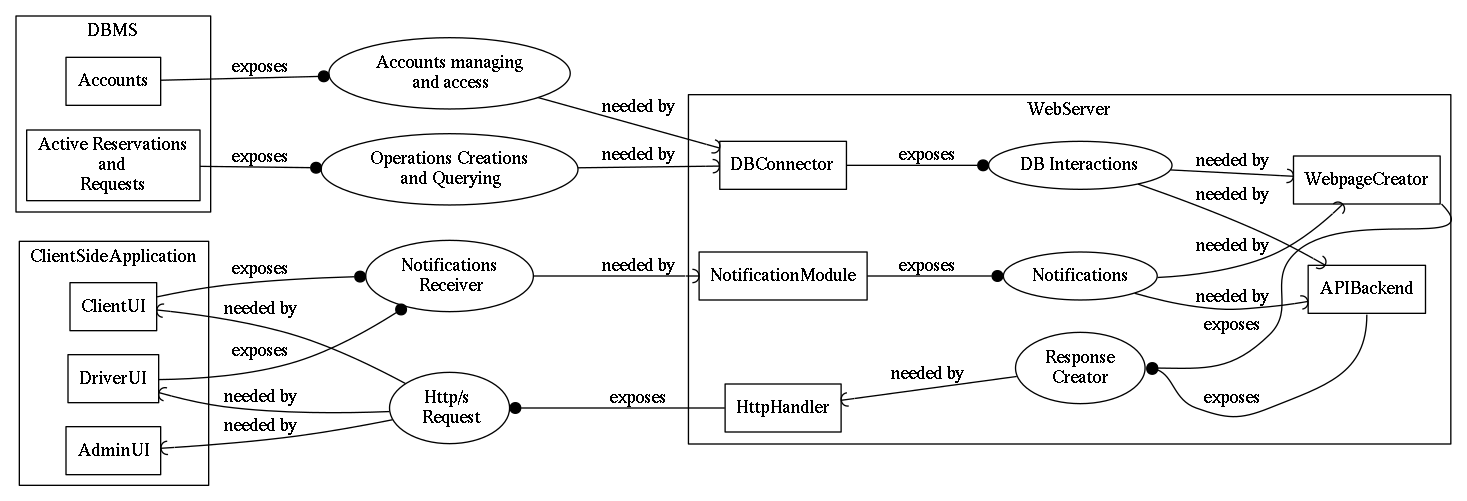
\includegraphics[width=1.4\textwidth]{Component}}%
\end{figure}
\subsection{Deployment View}
\begin{figure}[H]
	  \makebox[\textwidth][c]{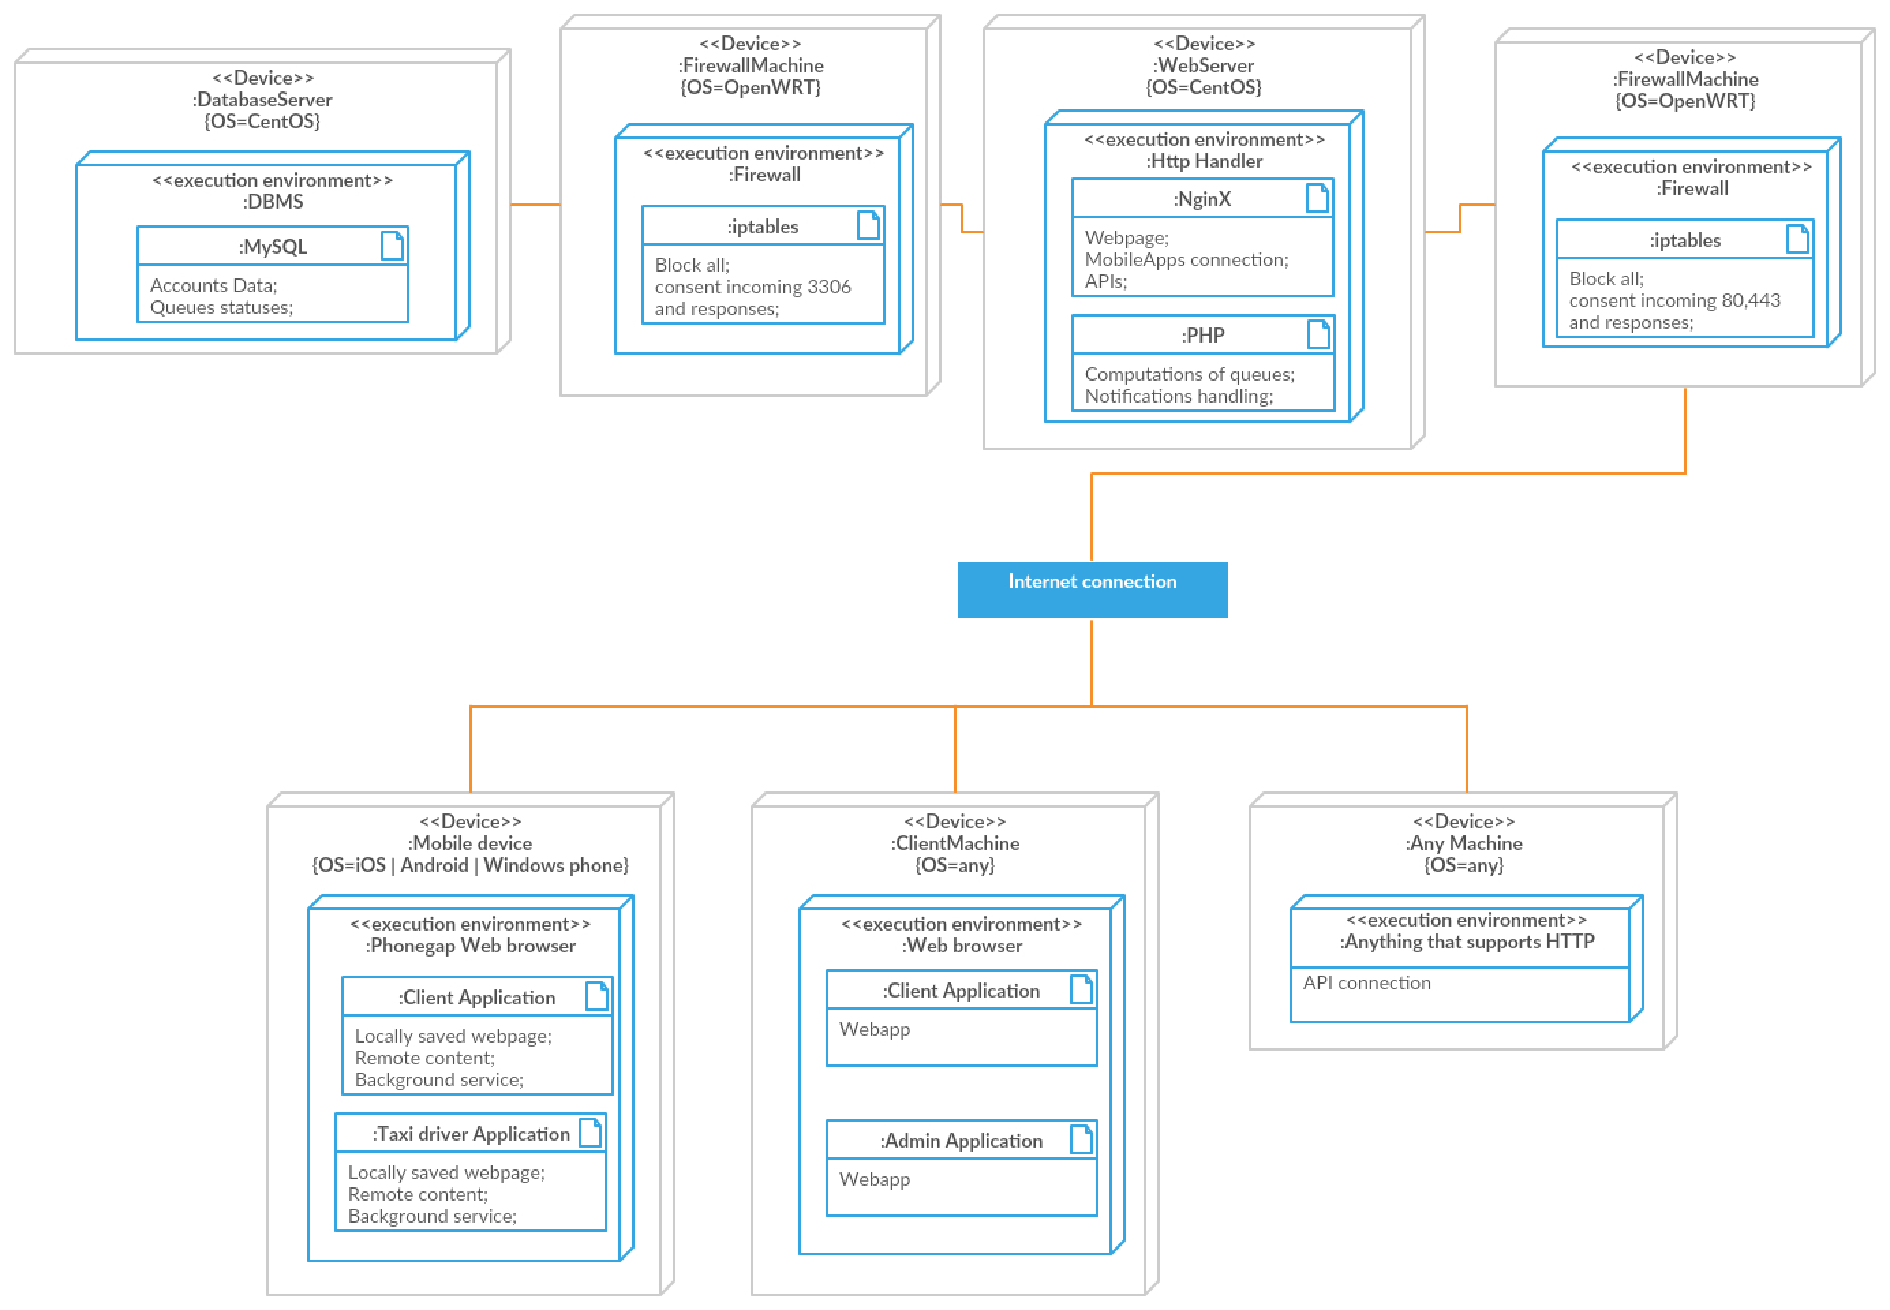
\includegraphics[width=1.3\textwidth]{Deployment}}%
\end{figure}
\subsection{Runtime View}
%sequence diagram
\subsection{Component Interfaces}
\paragraph{DBConnector}
The DBConnector encapsulates and exposes all the operations the Web Server needs to interact with the Database. The operations are divided in 2 categories based on the part of the Database they manage:
\begin{itemize}	
	\item Accounts: this component exposes methods to manage the stored end users accounts.
	
		\begin{tabular}{1*{3}{c}}
			\toprule
			Method & Parameters required & Notes \\
			\midrule
			addAccount & type of the account, credentials & adds an account to the DB \\ %TODO finire
			modifyAccount & DB key, attribute to modify, new value of the attribute & \\ %TODO finire
			deleteAccount & & \\
			getAccount & DB key & returns the account corresponding to the key  \\
			%TODO aggiungere un getTable che fa vedere quali sono i campi del db?
			\bottomrule
		\end{tabular}
	
	
	
	
	
	
	
	\begin{itemize}
		\item 
	\end{itemize}	
	\item Active Reservations and Requests:
	\begin{itemize}
		\item
	\end{itemize}
	
\end{itemize}
\subsection{Selected Architectural Styles and Patterns}
%client-server
\subsection{Other Design Decisions}
%


\section{User Interface Design}
This section has been explored in RASD's section 2.1.1 ``User Interfaces'' so we refer to that one.

\section{Requirements Traceability}
%Explain	 how the requirements you have defined in  the RASD map	 into the design	 elements that you have  defined in this document

\section{References}
\clearpage
\section{Appendix}
Appendix for Roberto Clapis\\
Work hours: 15
\begin{center}
	Software Used:\\
	\-\\
	\begin{tabular}{*{2}{c}}
		\toprule
		Task & Software \\
		\midrule
		Edit \LaTeX\ Source & Vim\\
		Edit Graphs Sources & Vim\\
		Edit sources for Sequence Diagrams & Vim\\
		Convert Sequence Diagrams to images & Quick Sequence Diagram Editor\\
		Generate and Raster directed graphs& Dot\\
		Generate and Raster undirected graphs& Fdp\\
		General images mangling and cropping & ImageMagick \& Shotwell\\
		Convert \LaTeX\ source to PDF & \LaTeX\-MK\\
		Spell Check & Aspell \\
		\LaTeX\ Check & LaCheck\\
		\bottomrule
	\end{tabular}
\end{center}
\-\\
\-\\
\begin{comment}
TODO Erica
Appendix for Erica Stella\\
Work hours: 40
\begin{center}
	Software Used:\\
	\-\\
	\begin{tabular}{*{2}{c}}
		\toprule
		Task & Software \\
		\midrule
		Edit \LaTeX\ Source & TexStudio\\
		Use Case Diagrams & Eclipse\\
		Class Diagram & Eclipse\\
		General images mangling and cropping & GIMP\\
		Mockup & Pencil\\
		\bottomrule
	\end{tabular}
\end{center}
\end{comment}
\end{document}
